\documentclass[11pt,a4paper]{article}

\usepackage[T1]{fontenc}
\usepackage[utf8]{inputenc}
\usepackage{lmodern}
\usepackage[a4paper,margin=1in]{geometry}
\usepackage{setspace}
\usepackage{amsmath,amssymb}
\usepackage{graphicx}
\usepackage{xcolor}
\usepackage{booktabs}
\usepackage{hyperref}
\usepackage{enumitem}
\usepackage{tikz}
\usetikzlibrary{arrows.meta,positioning,shapes.geometric,fit,calc,backgrounds}

\hypersetup{colorlinks=true,linkcolor=blue,urlcolor=blue,citecolor=blue}
\setstretch{1.08}
\setlist[itemize]{leftmargin=1.5em}
\setlist[enumerate]{leftmargin=1.8em}

\newcommand{\repo}[1]{\texttt{#1}}

\newcommand{\safeimage}[3]{%
  \IfFileExists{#1}{%
    \includegraphics[width=#2]{#1}%
  }{%
    \fbox{\parbox[c][0.20\textheight][c]{#2}{\centering\small #3\\[0.4em]\footnotesize(Generate the figure by running the corresponding script.)}}%
  }%
}

\title{Reconstructed Workflow of the Thesis Workspace}
\author{Workspace Audit Report}
\date{24 April 2026}

\begin{document}
\maketitle

\begin{abstract}
This document summarizes the technical workflow implemented in the workspace by reading the project structure, scripts, and configuration files.
It explains the sequence of modeling, simulation, processing, imaging, inversion, and uncertainty analysis steps, and it links these steps to concrete folders and Python entry points.
In particular, the \repo{Diffraction\_Experiment} branch is framed as a \textit{detection} campaign for subwavelength change visibility, while the remaining inversion and Bayesian branches are framed as \textit{inference} pipelines for parameter recovery.
The report is reconstructed from available files, so it represents the implemented pipeline rather than an exact historical execution log.
\end{abstract}

\section{Workspace-Level View}

\begin{figure}[h!]
\centering
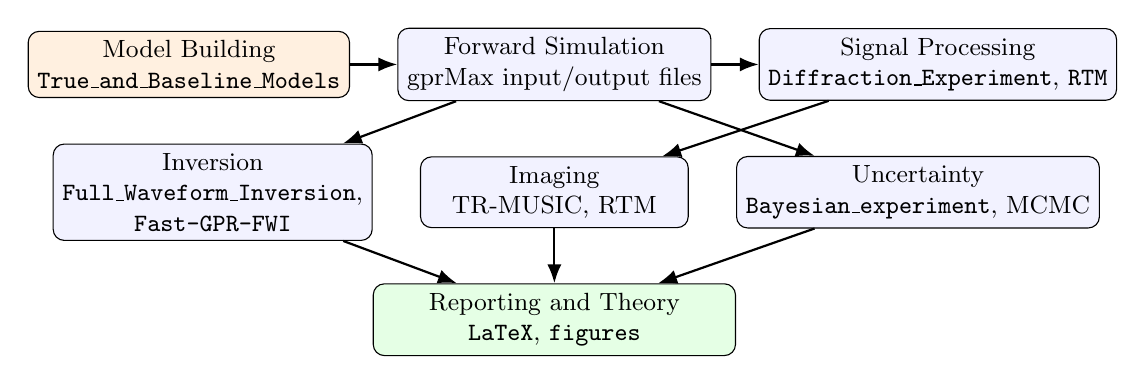
\begin{tikzpicture}[
    font=\small,
    node distance=7mm and 6mm,
    box/.style={draw, rounded corners, align=center, minimum height=8mm, minimum width=34mm, fill=blue!5},
    core/.style={box, fill=orange!12},
    arrow/.style={-{Latex[length=2.4mm]}, thick}
]
\node[core] (model) {Model Building\\\repo{True\_and\_Baseline\_Models}};
\node[box, right=of model] (sim) {Forward Simulation\\gprMax input/output files};
\node[box, right=of sim] (proc) {Signal Processing\\\repo{Diffraction\_Experiment}, \repo{RTM}};
\node[box, below=of sim] (img) {Imaging\\TR-MUSIC, RTM};
\node[box, left=of img] (inv) {Inversion\\\repo{Full\_Waveform\_Inversion},\\\repo{Fast-GPR-FWI}};
\node[box, right=of img] (bayes) {Uncertainty\\\repo{Bayesian\_experiment}, MCMC};
\node[box, below=of img, minimum width=46mm, fill=green!10] (thesis) {Reporting and Theory\\\repo{LaTeX}, \repo{figures}};

\draw[arrow] (model) -- (sim);
\draw[arrow] (sim) -- (proc);
\draw[arrow] (proc) -- (img);
\draw[arrow] (img) -- (thesis);
\draw[arrow] (sim) -- (inv);
\draw[arrow] (inv) -- (thesis);
\draw[arrow] (sim) -- (bayes);
\draw[arrow] (bayes) -- (thesis);
\end{tikzpicture}
\caption{High-level architecture of the workspace workflow.}
\label{fig:workspace-map}
\end{figure}

\section{Step-by-Step Technical Process}

\subsection*{Step 1: Define Physics and Resolution Constraints}
The utility functions in \repo{True\_and\_Baseline\_Models/helper.py} encode key physical constraints:
\begin{itemize}
    \item Central wavelength in a dielectric medium,
    \item Sub-wavelength fracture thickness threshold,
    \item Depth constraints and lateral resolution heuristics.
\end{itemize}
This indicates that the workflow starts from theoretical detectability limits before simulation setup.

\subsection*{Step 2: Build Baseline and True/Monitor Models}
The folder \repo{True\_and\_Baseline\_Models} contains baseline and process models (for example, \repo{baseline\_model.in}, \repo{process\_model.in}), with helpers to modify fracture geometry and material properties.
The script \repo{update\_aperture.py} exposes aperture sweeps via command-line arguments, which suggests controlled parametric studies on thin-bed/fracture geometry.

\subsection*{Step 3: Run Forward Simulations (gprMax)}
Multiple subprojects generate and run gprMax files:
\begin{itemize}
    \item \repo{RTM/generate\_and\_run.py} creates a multi-shot acquisition over subwavelength scatterers,
    \item \repo{Diffraction\_Experiment/run\_simulation\_and\_plot.py} triggers forward simulations and immediate plotting,
    \item \repo{Diffraction\_Experiment/run\_multi\_tx\_trmusic.py} automates multi-transmitter data acquisition.
\end{itemize}
At this stage, raw \repo{.out} files are produced for both target and homogeneous/baseline scenarios.

\subsection*{Step 4: Differential Data Construction}
A recurring pattern in the code is subtraction of baseline/homogeneous responses from target responses to isolate weak scattered components:
\[
\delta d(t, x_{tx}, x_{rx}) = d_{\mathrm{target}}(t, x_{tx}, x_{rx}) - d_{\mathrm{baseline}}(t, x_{tx}, x_{rx}).
\]
This differential strategy appears in RTM and TR-MUSIC pipelines and is also consistent with the MCMC plan in \repo{LaTeX/plan.tex}.

\subsection*{Step 5: Advanced Signal Processing and Feature Enhancement}
The object-oriented workflow in \repo{Diffraction\_Experiment/processing\_OO.py} and \repo{run\_simulation\_and\_plot.py} applies:
\begin{itemize}
    \item wiggle-trace diagnostics,
    \item auto/cross-correlation,
    \item CWT amplitude and phase imaging,
    \item phase derivatives (time and frequency),
    \item geometric shift-and-correlate with XWT.
\end{itemize}
This reveals a strong emphasis on extracting subtle diffraction signatures and phase behavior as a \textbf{detection} problem: the objective is to determine whether a subwavelength perturbation is observable above background and direct-wave clutter.

\subsection*{Step 6: Imaging with TR-MUSIC and RTM}
Two imaging routes coexist:
\begin{itemize}
    \item \textbf{TR-MUSIC branch}: \repo{Diffraction\_Experiment/trmusic\_diffraction.py} and multi-Tx runners,
    \item \textbf{RTM branch}: \repo{RTM/process\_rtm.py} (frequency-domain reflection matrix backpropagation with FMC geometry).
\end{itemize}
Both branches transform processed multistatic data into spatial focusing maps of likely scatterer locations.

\subsection*{Step 6.5: Detection Branch vs Inference Branches}
The project is split into two methodological goals:
\begin{itemize}
    \item \textbf{Detection goal (Diffraction\_Experiment):} establish whether subwavelength changes produce statistically and visually separable signatures in differential traces, CWT/XWT maps, and TR-MUSIC pseudo-spectra.
    \item \textbf{Inference goal (other folders):} estimate physical parameters (for example aperture, permittivity, conductivity, or velocity-related fields) using optimization or Bayesian posterior sampling.
\end{itemize}
In short, \repo{Diffraction\_Experiment} answers \textit{``Can we see it?''} and the inversion/Bayesian branches answer \textit{``What is it?''}.

\subsection*{Step 7: Full Waveform Inversion (FWI)}
The folder \repo{Full\_Waveform\_Inversion} contains a Devito-based inversion stack:
\begin{itemize}
    \item forward/adjoint operator construction,
    \item objective and gradient evaluation,
    \item bounded L-BFGS-B optimization,
    \item data preparation scripts and plotting utilities.
\end{itemize}
The script \repo{run\_fwi.py} includes explicit Windows compatibility patches for Devito memory allocation and compilation paths, confirming active adaptation to the local OS environment.

\subsection*{Step 8: Accelerated Dual-Parameter FWI (GPU/PyTorch/CUDA)}
The folder \repo{Fast-GPR-FWI} introduces a second inversion track focused on speed and dual-parameter recovery (permittivity and conductivity), with CUDA-accelerated kernels integrated into PyTorch according to \repo{Fast-GPR-FWI/README.md}.

\subsection*{Step 9: Bayesian Inference and Uncertainty Quantification}
The script \repo{Bayesian\_experiment/Bayesian\_inference.py} implements a Metropolis-Hastings loop:
\begin{itemize}
    \item propose fracture parameter values,
    \item regenerate gprMax input,
    \item run simulation,
    \item compare with observed data through a Gaussian likelihood.
\end{itemize}
This yields posterior traces for model parameters and complements deterministic inversion with uncertainty estimates.

\subsection*{Step 10: Alternative Misfit Research Track}
The folder \repo{Quantum\_Geometric\_Misfits-main} contains scripts for L2 and geometric/quantum-inspired misfit experiments, including batch execution via \repo{run\_in\_sequence.py}.
This indicates method-comparison work beyond classical least-squares objectives.

\section{Diffraction\_Experiment as a Detection Campaign}

The folder \repo{Diffraction\_Experiment} is the dedicated observability testbed for subwavelength change detection.
Its internal structure maps naturally to a detection workflow:
\begin{itemize}
    \item \repo{forward.py}: build and run alternating and homogeneous forward models.
    \item \repo{processing.py}, \repo{processing\_OO.py}: construct differential traces and apply signal conditioning (correlation, wavelet analysis, phase diagnostics).
    \item \repo{plotting.py}, \repo{plotting\_OO.py}: produce diagnostic figures used to decide if change-related energy is resolvable.
    \item \repo{run\_simulation\_and\_plot.py}: end-to-end driver for simulation + detection analytics.
    \item \repo{run\_multi\_tx\_trmusic.py}, \repo{run\_multi\_tx\_trmusic\_gapped.py}, \repo{trmusic\_diffraction.py}: multi-Tx acquisition and TR-MUSIC pseudo-spectrum imaging for location-level detectability.
    \item \repo{horizontal\_scattering\_0p5lambda\_snaps}, \repo{horizontal\_scattering\_homogeneous\_snaps}: forward-wavefield snapshots for qualitative comparison.
    \item \repo{cwt\_3d\_traces}: per-trace wavelet images for trace-by-trace detectability checks.
\end{itemize}

\begin{figure}[h!]
\centering
\begin{minipage}{0.49\textwidth}
\centering
\safeimage{Diffraction_Experiment/gpr_snapshots_result_diff_traces.png}{0.98\linewidth}{Differential traces from forward snapshots}
\end{minipage}
\hfill
\begin{minipage}{0.49\textwidth}
\centering
\safeimage{Diffraction_Experiment/plot_diff_raw.png}{0.98\linewidth}{Differential wiggle traces}
\end{minipage}

\vspace{0.6em}

\begin{minipage}{0.49\textwidth}
\centering
\safeimage{Diffraction_Experiment/plot_diff_cwt.png}{0.98\linewidth}{Global differential CWT magnitude}
\end{minipage}
\hfill
\begin{minipage}{0.49\textwidth}
\centering
\safeimage{Diffraction_Experiment/plot_diff_xwt_t11_t12.png}{0.98\linewidth}{XWT coherence/phase for a trace pair}
\end{minipage}
\caption{Detection-oriented diagnostics in \repo{Diffraction\_Experiment}: differential response isolation, time-frequency concentration, and inter-trace phase coherence.}
\label{fig:diff-detection-panels}
\end{figure}

\begin{figure}[h!]
\centering
\safeimage{RTM/trmusic_result_fmc.png}{0.72\linewidth}{TR-MUSIC detection map (FMC)}
\caption{TR-MUSIC pseudo-spectrum using the requested FMC result image, used as a detectability indicator for subwavelength perturbations.}
\label{fig:diff-trmusic-detect}
\end{figure}

\section{Core Research Loop}

\begin{figure}[h!]
\centering
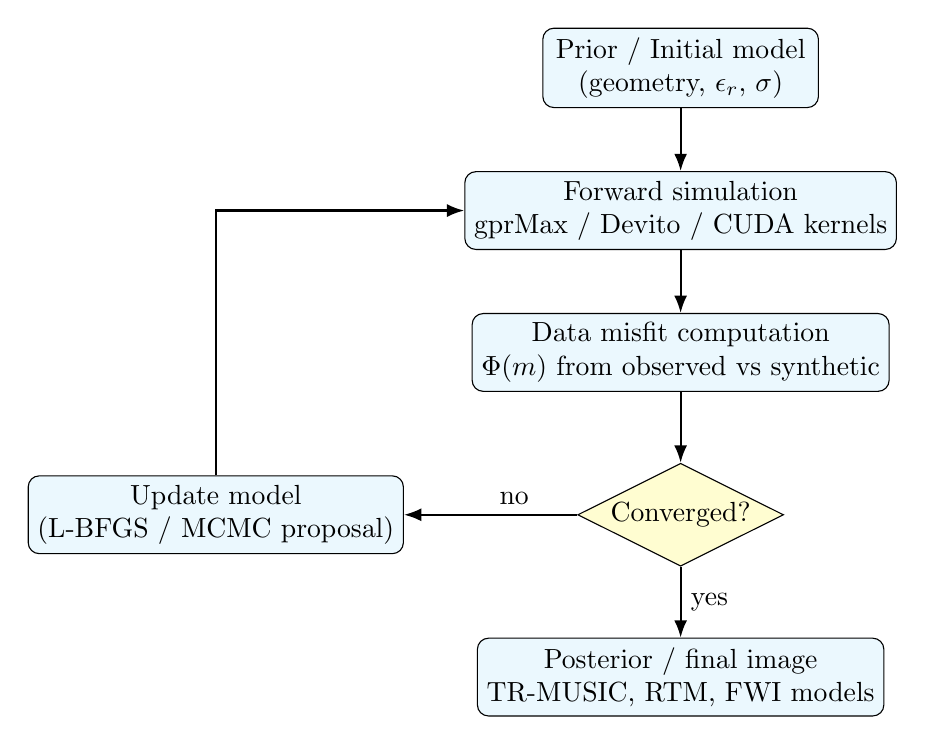
\begin{tikzpicture}[
    node distance=8mm and 7mm,
    block/.style={draw, rounded corners, align=center, minimum width=35mm, minimum height=8mm, fill=cyan!8},
    decision/.style={draw, diamond, aspect=2.0, align=center, inner sep=1pt, fill=yellow!18},
    arrow/.style={-{Latex[length=2.2mm]}, thick}
]
\node[block] (prior) {Prior / Initial model\\(geometry, $\epsilon_r$, $\sigma$)};
\node[block, below=of prior] (forward) {Forward simulation\\gprMax / Devito / CUDA kernels};
\node[block, below=of forward] (misfit) {Data misfit computation\\$\Phi(m)$ from observed vs synthetic};
\node[decision, below=of misfit, yshift=-1mm] (accept) {Converged?};
\node[block, left=22mm of accept] (update) {Update model\\(L-BFGS / MCMC proposal)};
\node[block, below=of accept, yshift=-1mm] (posterior) {Posterior / final image\\TR-MUSIC, RTM, FWI models};

\draw[arrow] (prior) -- (forward);
\draw[arrow] (forward) -- (misfit);
\draw[arrow] (misfit) -- (accept);
\draw[arrow] (accept) -- node[right]{yes} (posterior);
\draw[arrow] (accept.west) -- ++(-8mm,0) node[above]{no} |- (update);
\draw[arrow] (update) |- (forward.west);
\end{tikzpicture}
\caption{Unified optimization/inference loop implemented across deterministic and Bayesian pipelines.}
\label{fig:core-loop}
\end{figure}

\section{Representative Outputs}

\begin{figure}[h!]
\centering
\begin{minipage}{0.48\textwidth}
\centering
\safeimage{RTM/rtm_result_fmc.png}{0.95\linewidth}{RTM image map}
\end{minipage}
\hfill
\begin{minipage}{0.48\textwidth}
\centering
\safeimage{RTM/trmusic_result_fmc.png}{0.95\linewidth}{TR-MUSIC FMC map}
\end{minipage}
\caption{Auto-loaded outputs if available; placeholders are shown otherwise.}
\label{fig:outputs}
\end{figure}

\section{Execution Timeline (Reconstructed)}

\begin{figure}[h!]
\centering
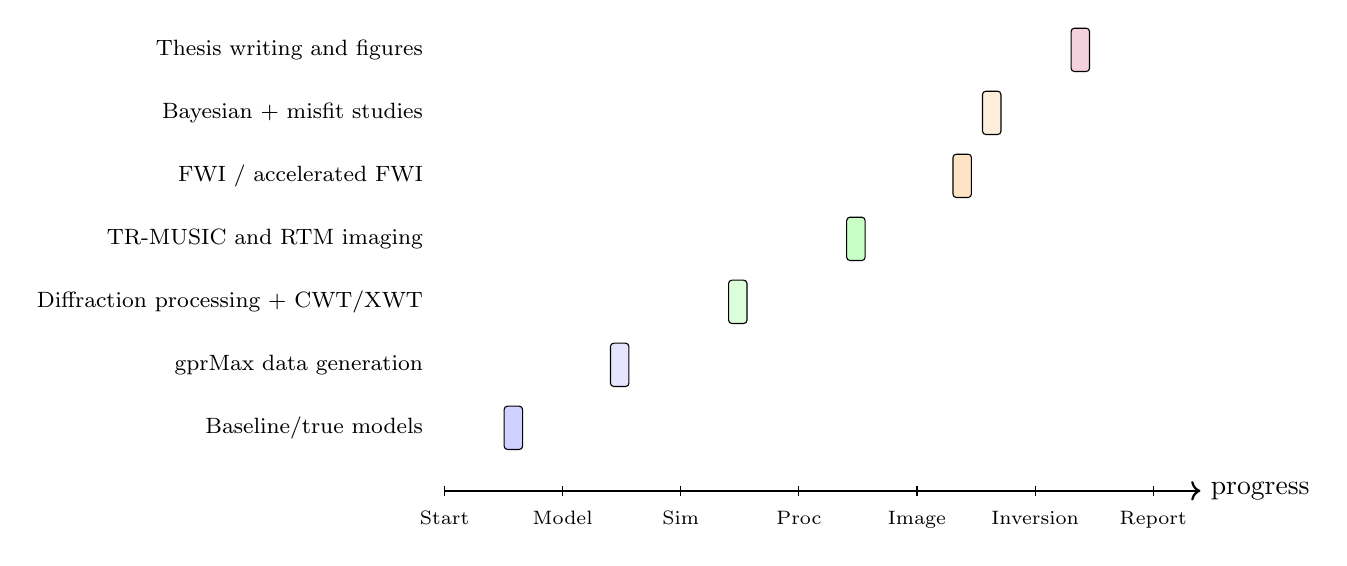
\begin{tikzpicture}[
    x=0.75cm,
    y=0.8cm,
    task/.style={draw, rounded corners=1.2pt, fill=gray!12, minimum height=0.55cm, anchor=west},
    label/.style={anchor=east, font=\footnotesize}
]
% Axis
\draw[->, thick] (0,0) -- (12.8,0) node[right] {progress};
\foreach \x/\txt in {0/Start,2/Model,4/Sim,6/Proc,8/Image,10/Inversion,12/Report} {
  \draw (\x,0.08) -- (\x,-0.08) node[below=2pt, font=\scriptsize] {\txt};
}

\node[label] at (-0.2,1.0) {Baseline/true models};
\node[task, fill=blue!18] at (1.0,1.0) {\hspace{2.9cm}};

\node[label] at (-0.2,2.0) {gprMax data generation};
\node[task, fill=blue!10] at (2.8,2.0) {\hspace{3.6cm}};

\node[label] at (-0.2,3.0) {Diffraction processing + CWT/XWT};
\node[task, fill=green!14] at (4.8,3.0) {\hspace{3.1cm}};

\node[label] at (-0.2,4.0) {TR-MUSIC and RTM imaging};
\node[task, fill=green!22] at (6.8,4.0) {\hspace{2.4cm}};

\node[label] at (-0.2,5.0) {FWI / accelerated FWI};
\node[task, fill=orange!22] at (8.6,5.0) {\hspace{2.0cm}};

\node[label] at (-0.2,6.0) {Bayesian + misfit studies};
\node[task, fill=orange!14] at (9.1,6.0) {\hspace{2.2cm}};

\node[label] at (-0.2,7.0) {Thesis writing and figures};
\node[task, fill=purple!18] at (10.6,7.0) {\hspace{1.6cm}};
\end{tikzpicture}
\caption{Reconstructed sequence of work packages across the repository.}
\label{fig:timeline}
\end{figure}

\section{Directory-to-Task Mapping}

\begin{table}[h!]
\centering
\small
\begin{tabular}{@{}p{0.30\textwidth}p{0.62\textwidth}@{}}
\toprule
Directory & Main role in the workflow \\
\midrule
\repo{True\_and\_Baseline\_Models} & Geometry design, baseline/process model generation, aperture and material parameter control. \\
\repo{Diffraction\_Experiment} & \textbf{Detection branch}: differential signal analysis, CWT/XWT feature extraction, and TR-MUSIC-based observability tests for subwavelength changes (``can we detect it?''). \\
\repo{RTM} & FMC survey generation and reflection-matrix-based RTM imaging. \\
\repo{Full\_Waveform\_Inversion} & Devito forward/adjoint operators and bounded L-BFGS inversion. \\
\repo{Fast-GPR-FWI} & CUDA + PyTorch accelerated dual-parameter FWI experiments. \\
\repo{Bayesian\_experiment} & Metropolis-Hastings parameter \textbf{inference} and posterior trace generation (``what is the change?''). \\
\repo{Quantum\_Geometric\_Misfits-main} & Alternative objective-function experiments (L2 and geometric tracks). \\
\repo{LaTeX} & Theory notes, planning, and manuscript/report material. \\
\bottomrule
\end{tabular}
\caption{How each major folder contributes to the end-to-end research process.}
\label{tab:dir-map}
\end{table}

\section{Closing Notes}
The workspace reflects a two-layer research strategy: a detection layer (centered on \repo{Diffraction\_Experiment}) to validate subwavelength observability, and an inference layer (FWI, accelerated FWI, Bayesian, and misfit-analysis branches) to estimate the underlying physical change once detectability is established.
A practical next step is to append run metadata (date, command, git commit hash, runtime, key parameters) to each experiment so future reports can be generated as exact execution logs.

\end{document}
